\documentclass[a4paper,12pt,french] {article}

\usepackage{../../../Style}

\pagestyle{empty}

\begin{document}

\entete{06/10/2021}{\textbf{Interrogation - Sujet A}}{\seconde 12}

\vspace{-5mm}

Nom: \hfill Prénom: \hfill \

\compolignehaut[0.5]
{
\begin{exercice}
Donner les trois caractéristiques d'un vecteur:

\begin{itemize}

\vspace{1cm}

\item \vspace{1cm}

\item \vspace{1cm}

\item \vspace{1cm}
\end{itemize}
\end{exercice}
}
{
\begin{exercice} \

\begin{center}
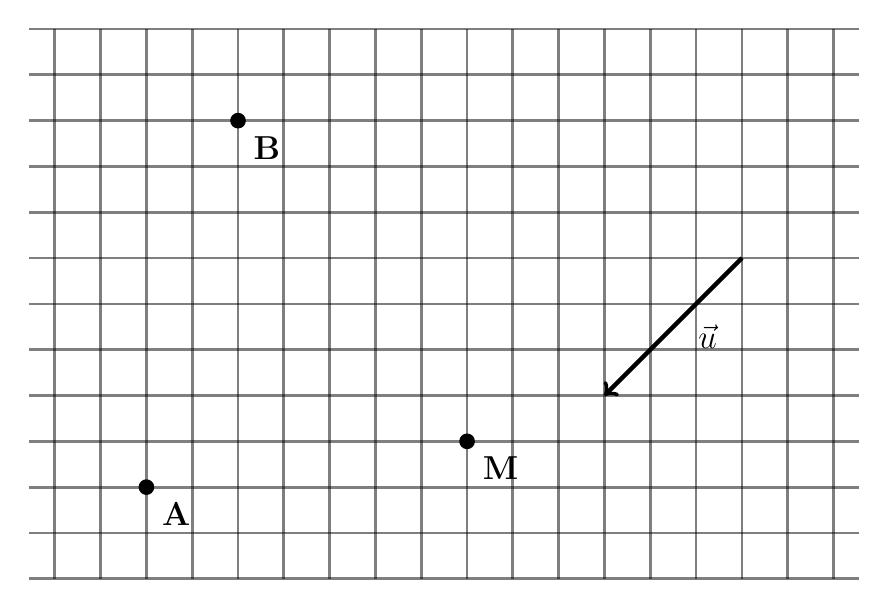
\begin{tikzpicture}[scale=1]
\begin{axis}[
%axis x line=bottom,
%axis y line = left,
%axis lines=middle,
width=\linewidth,
height=\pgfkeysvalueof{/pgfplots/width}*((\pgfkeysvalueof{/pgfplots/ymax})+((-1)*(\pgfkeysvalueof{/pgfplots/ymin})))/((\pgfkeysvalueof{/pgfplots/xmax})+((-1)*(\pgfkeysvalueof{/pgfplots/xmin})))+0.1pt,
xmin=0, xmax=17,
ymin=0, ymax=12,
%enlargelimits={abs=0.2},
xtick distance=1,
ytick distance=1,
grid=both,
xticklabels={},
yticklabels={},
grid style={black,line width=1pt, draw opacity=0.5},
ticks=none,
axis equal,
legend pos=north east,
axis line style={draw=none},
scale=1,
]
\node[color=black,circle,minimum size=1pt,fill,inner sep=2pt,fill opacity=1,label={-45:\textbf{\large A}}] (A) at (2,2) {};
\node[color=black,circle,minimum size=1pt,fill,inner sep=2pt,fill opacity=1,label={-45:\textbf{\large B}}] (B) at (4,10) {};
\node[color=black,circle,minimum size=1pt,fill,inner sep=2pt,fill opacity=1,label={-45:\textbf{\large M}}] (B) at (9,3) {};
\draw[ultra thick,color=black,->] (15,7) -- (12,4) node[pos=0.4,below right] {\large $\vec u$};

\end{axis}
\end{tikzpicture}
\end{center}

\begin{enumerate}
\item Placer $N$, l'image de $M$ par la translation de vecteur $\vecc {AB}$.
\item Tracer un représentant du vecteur $\vec u$ ayant pour origine le point $B$.
\end{enumerate}
\end{exercice}
}

\vfill

\setcounter{exercice} 0

\entete{06/10/2021}{\textbf{Interrogation - Sujet B}} {\seconde 12}

\vspace{-5mm}

Nom: \hfill Prénom: \hfill \

\compolignehaut[0.4]
{
\begin{exercice}
Donner les trois caractéristiques d'un vecteur:

\begin{itemize}

\vspace{1cm}

\item \vspace{1cm}

\item \vspace{1cm}

\item \vspace{1cm}
\end{itemize}

\end{exercice}
}
{
\begin{exercice} \
\begin{center}
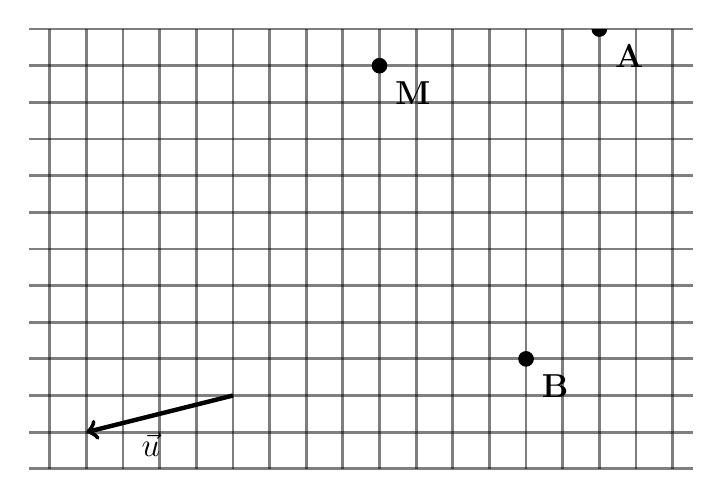
\begin{tikzpicture}[scale=1]
\begin{axis}[
%axis x line=bottom,
%axis y line = left,
%axis lines=middle,
width=\linewidth,
height=\pgfkeysvalueof{/pgfplots/width}*((\pgfkeysvalueof{/pgfplots/ymax})+((-1)*(\pgfkeysvalueof{/pgfplots/ymin})))/((\pgfkeysvalueof{/pgfplots/xmax})+((-1)*(\pgfkeysvalueof{/pgfplots/xmin})))+0.1pt,
xmin=0, xmax=17,
ymin=0, ymax=12,
%enlargelimits={abs=0.2},
xtick distance=1,
ytick distance=1,
grid=both,
xticklabels={},
yticklabels={},
grid style={black,line width=1pt, draw opacity=0.5},
ticks=none,
axis equal,
legend pos=north east,
axis line style={draw=none},
scale=0.8
]
\node[color=black,circle,minimum size=1pt,fill,inner sep=2pt,fill opacity=1,label={-45:\textbf{\large A}}] (A) at (15,12) {};
\node[color=black,circle,minimum size=1pt,fill,inner sep=2pt,fill opacity=1,label={-45:\textbf{\large B}}] (B) at (13,3) {};
\node[color=black,circle,minimum size=1pt,fill,inner sep=2pt,fill opacity=1,label={-45:\textbf{\large M}}] (M) at (9,11) {};
\draw[ultra thick,color=black,->] (5,2) -- (1,1) node[pos=0.7,below right] {\large $\vec u$};

\end{axis}
\end{tikzpicture}
\end{center}

\begin{enumerate}
\item Placer $N$, l'image de $M$ par la translation de vecteur $\vecc {AB}$.
\item Tracer un représentant du vecteur $\vec u$ ayant pour origine le point $M$.
\end{enumerate}
\end{exercice}
}

\vfill

\end{document}
